%!TEX program = pdflatex
% Full chain: pdflatex -> bibtex -> pdflatex -> pdflatex
\documentclass[11pt]{elegantpaper}

\title{TSP 问题及其求解\\ {\small 开题报告}}
\author{\href{https://github.com/LT1st/System_engineering_programm/tree/master}{ 卢韬 }}
\institute{\href{https://github.com/ElegantLaTeX}{自动化1903班 20194127}}
%\version{0.07}
%\date{\today}


\begin{document}

\maketitle

\begin{abstract}
\noindent 
\qquad TSP问题已经被研究多年【引用综述文献】,已有诸多工作从精确算法【动态规划】、启发式算法【随机贪婪搜索】、元启发式算法【遗传算法、粒子群优化算法】等方向入手,并在获取精确解的能力上取得了较好的效果。然而,由于TSP问题NP难的特点,没有单一的方法能快速、精确地求解各种类型的TSP样例。而这些算法评价指标之间普遍存在着诸多trade-off,单一的求解最优解的能力不足以衡量算法好坏。
因此面对不同特点的算例样本,需要一种科学的评价指标衡量选取哪种算法更好。
本项目将讨论多种用于求解TSP问题算法的原理,并将使用python复现、对比各类算法。最终,结合实验过程和关键评价指标(精度、复杂度、速度)给出一种统一的算法评价指标计算方法,并得到不同特点的算例下最适合的算法。
所有的代码和笔记将开源在:
%引文
\href{https://github.com/LT1st/System_engineering_programm/tree/master}{github开源地址}。\par
\keywords{TSP问题,遗传算法,禁忌搜索,贪婪算法,动态规划算法,粒子群优化算法}
\end{abstract}

\newpage
\tableofcontents
\newpage

\section{TSP问题介绍}

This template is based on the standard \LaTeX{} article class, which means you can pass the arguments of article class to it (\lstinline{a4paper}, \lstinline{10pt} and etc.)( \lstinline{11pt} is recommended). It supports different engines, You can choose either \lstinline{PDFLaTeX} or \lstinline{XeLaTeX}\footnote{with \lstinline{ctex} package for Chinese fonts settings.}. 

对TSP问题有如下数学描述:
\begin{equation}
\min \sum_{i,j=1}^{n} x_{ij} d_{ij} \label{eq:binom}
\end{equation}

其中约束为:
\begin{equation}
\sum_{i\in V} x_{i j}=1 , \forall i \in V_{c}
\label{eq:binom}
\end{equation}

\begin{equation}
\sum_{j\in V} x_{i j}=1 , \forall j \in V_{c}
\label{eq:binom}
\end{equation}

\begin{equation}
\sum_{i\in S} \sum_{j\in S} x_{i j}\leq \lvert S \rvert - 1  ,\quad \forall S \subset V_{c} , 2 \leq \lvert S \lrvert \leq n
\label{eq:binom}
\end{equation}

公式中的未知数为:
\begin{table}[htbp]
  \small
  \centering%居中
  \caption{未知数含义 \label{tab:reg}}
    \begin{tabular}{cccc}%表示行数、居中方式
    \toprule
        未知数    &  含义         &        取值范围    &  注释  \\
    \midrule
    d_{i j}     &    i到j的距离  &   [0,-\infty)   &  距离衡量可以用p范数  \\
    x_{i j}     &   在i后访问j   &      0,1         & 使用one-hot编码 \\
    i , j       &   城市代号     &  i \neq j        & 城市数量          \\
    \bottomrule
    %\multicolumn{4}{l}{\scriptsize Standard errors in parentheses} \\
    %\multicolumn{4}{l}{\scriptsize *** p<0.01, ** p<0.05, * p<0.1} \\
    \end{tabular}%
\end{table}%

\subsection{Global Options}
I defined one option named \lstinline{lang}, this option has two alternative values, \lstinline{lang=en} (default) or \lstinline{lang=cn}. \lstinline{lang=cn} will make the caption of figure/table, abstract name, refname etc. Chinese, while \lstinline{lang=en} will keep all these stuff English, as the default article class sets. You can use this option as

\begin{lstlisting}
\documentclass[lang=en]{elegantpaper}
\documentclass{en}{elegantpaper} % both ok
\end{lstlisting}

\subsection{Custom Commands}

I don't change any default command or environment, which means you can use all the basic \LaTeX{} commands and environments as before.  Besides, I define 3 commands
\begin{enumerate}
	\item \lstinline{\email}: create the hyperlink to email address.
	\item \lstinline{\figref}: same usage as \lstinline{\ref}, but start with label text <\textbf{Figure n}>.
	\item \lstinline{\tabref}: same usage as \lstinline{\ref}, but start with label text <\textbf{Table n}>.
	\item \lstinline{\keywords}: create the keywords in the abstract section.
\end{enumerate}{}

\subsection{List Environments}
You can use \lstinline{itemize}, \lstinline{enumerate}, or \lstinline{description} environment as below\\
\begin{minipage}[c]{0.51\linewidth}
\begin{lstlisting}
\begin{itemize}
    \item Routing and resource discovery;
    \item Resilient and scalable networks;
    \item Distributed storage and search.
\end{itemize}
\end{lstlisting}
\end{minipage}
\begin{minipage}[c]{0.48\linewidth}
\begin{itemize}
    \item Routing and resource discovery;
    \item Resilient and scalable networks;
    \item Distributed storage and search.
\end{itemize}
\end{minipage}

\subsection{Table}
I strongly recommend you to use the \lstinline{booktabs} package in your paper. It adds three commands to make the table prettier, ie. \lstinline{\toprule}, \lstinline{\midrule} and \lstinline{\bottomrule}. \tabref{tab:reg} is an example.

\begin{lstlisting}
\begin{table}[htbp]
  \small
  \centering
  \caption{Auto MPG and Price \label{tab:reg}}
    \begin{tabular}{lcc}
    \toprule
                    &       (1)         &        (2)      \\
    \midrule
    mpg             &    -238.90***     &      -49.51     \\
                    &     (53.08)       &      (86.16)    \\
    weight          &                   &      1.75***    \\
                    &                   &      (0.641)    \\
    constant        &     11,253***     &       1,946     \\
                    &     (1,171)       &      (3,597)    \\
    obs             &        74         &         74      \\
    $R^2$           &      0.220        &       0.293     \\
    \bottomrule
    \multicolumn{3}{l}{\scriptsize Standard errors in parentheses} \\
    \multicolumn{3}{l}{\scriptsize *** p<0.01, ** p<0.05, * p<0.1} \\
    \end{tabular}%
\end{table}%
\end{lstlisting}
\begin{table}[htbp]
  \small
  \centering
  \caption{Auto MPG and Price \label{tab:reg}}
    \begin{tabular}{lcc}
    \toprule
                    &       (1)         &        (2)      \\
    \midrule
    mpg             &    -238.90***     &      -49.51     \\
                    &     (53.08)       &      (86.16)    \\
    weight          &                   &      1.75***    \\
                    &                   &      (0.641)    \\
    constant        &     11,253***     &       1,946     \\
                    &     (1,171)       &      (3,597)   \\
    obs             &        74         &         74     \\
    $R^2$           &      0.220        &       0.293    \\
    \bottomrule
    \multicolumn{3}{l}{\scriptsize Standard errors in parentheses} \\
    \multicolumn{3}{l}{\scriptsize *** p<0.01, ** p<0.05, * p<0.1} \\
    \end{tabular}%
\end{table}%



\subsection{Graphics}
To include a graphic, you can use figure environment as usual. \figref{fig:scatter} shows the effect. You can put all your images in the sub directories (\lstinline{./image/}, \lstinline{./img/}, \lstinline{./figure/}, \lstinline{./fig/}) of your current working directory.

\begin{lstlisting}
\begin{figure}[htbp]
	\centering
	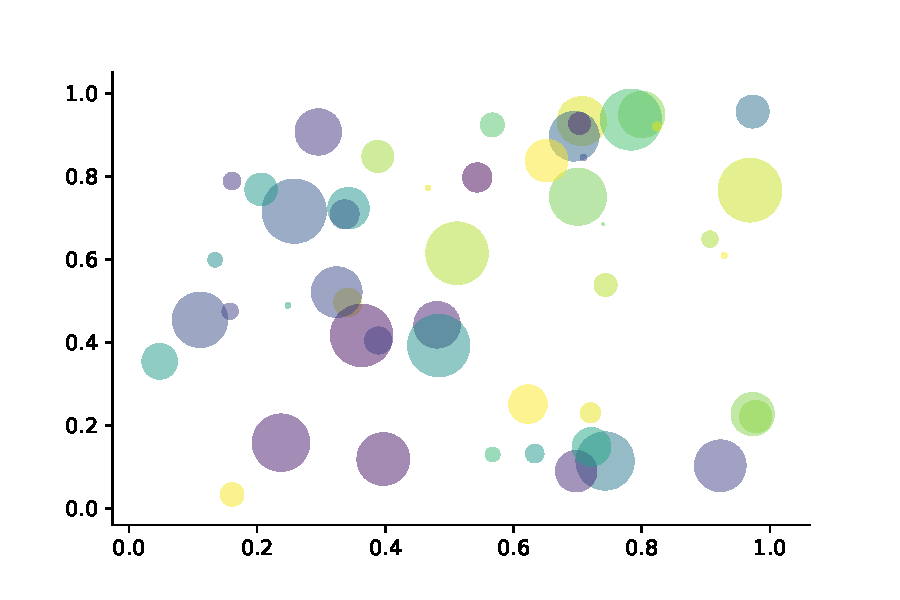
\includegraphics[width=0.6\textwidth]{scatter.pdf}
	\caption{Scatter Plot Example \label{fig:scatter}}
\end{figure}
\end{lstlisting}
\begin{figure}[htbp]
	\centering
	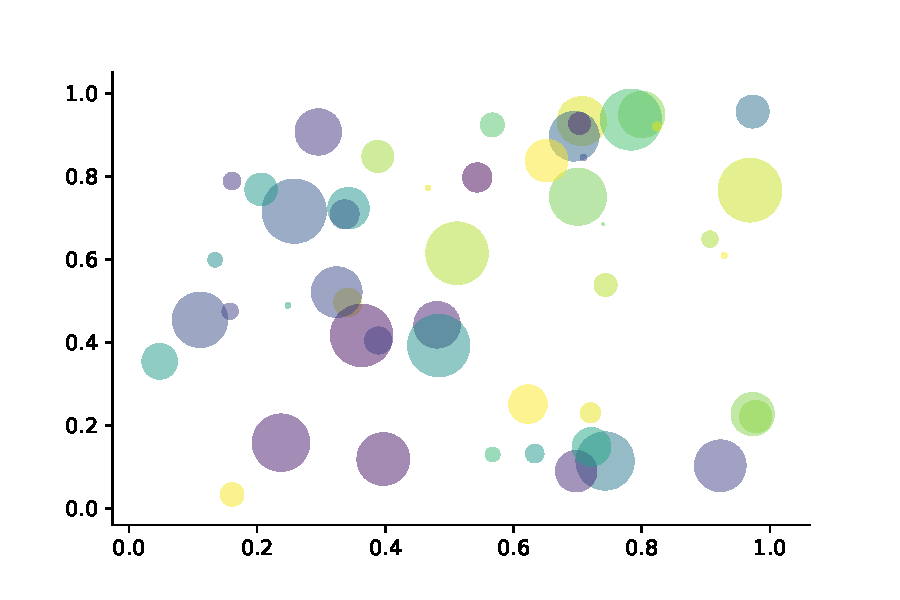
\includegraphics[width=0.6\textwidth]{scatter.pdf}
	\caption{Scatter Plot Example \label{fig:scatter}}
\end{figure}

\subsection{Bibliography}
This template uses Bib\TeX{} to generate the bibliography, the default bibliography style is \lstinline{unsrt}. Let's take a glance at the citation effect, ~\cite{en3} use data from a major peer-to-peer lending marketplace in China to study whether female and male investors evaluate loan performance differently. 

If you want to use Bib\TeX{}, you must create a file named \lstinline{wpref.bib}, and add bib items (from Google Scholar, Mendeley, EndNote, and etc.) to \lstinline{wpref.bib} file, and cite the bibkey in the \lstinline{tex} file. The Bib\TeX{} will automatically generate the bibliography for you for the reference you cited. If you want to add some noncited references or all of them to the bibliography,  you can use 

\begin{lstlisting}
\nocite{EINAV2010, Havrylchyk2018} % add two noncited references 
\nocite{*} % list all the references of the bib file.
\end{lstlisting}

If you want to change the bibliography style, you can replace \lstinline{aer} for the prefered style, for example, the \lstinline{unsrt} style.

\begin{lstlisting}
\bibliographystyle{unsrt}
\end{lstlisting}

\section{A Minimal Example}
In this section, we give a simple example using this template.

\begin{lstlisting}
\documentclass[lang=en]{elegantpaper}

% title information
\title{A Working Paper Example}
\author{ddswhu} 
\institute{Elegant\LaTeX{} Group}
\version{1.00}
\date{\today}

\begin{document}

\maketitle

\begin{abstract}
Your abstract goes here.
\keywords{keyword1, keyword2}
\end{abstract}

\section{Introduction}
The content of introduction section.

\section{Conclusion}
The content of conclusion section.

% include the noncited reference
\nocite{ref1, ref2}
\bibliographystyle{aer}
\bibliography{wpref}
\end{document}
\end{lstlisting}

\nocite{en1,en2}

% If you want change the bibliography style, replace aer with the prefered one.
\bibliographystyle{aer}

\bibliography{wpref}%导入bib包,这是包的名字

\end{document}
